\section{Caracterização de mudanças de caminhos}
\label{sec:char}

Nesta seção caracterizamos um conjunto de mudanças de caminho reais e
verificamos que mudanças de caminho na Internet afetam poucos
roteadores.

Implantamos o \dtrack{}~\cite{cunha11dtrack} para medir caminhos em 72
monitores no PlanetLab por uma semana a partir de 4 de março de 2011.
Cada monitor escolhe 1.000 destinos aleatoriamente de uma lista com
34.820 destinos alcançáveis escolhidos aleatoriamente na Internet.  Em
cada monitor, configuramos o \dtrack{} para rastrear mudanças nos
caminhos escolhidos enviando 8 sondas por segundo, similar à taxa de
sondagem do DIMES~\cite{shavitt09dimes}.  Em uma semana observamos
1.202.960 mudanças de caminho.  Os caminhos medidos atravessam 7.315
sistemas autônomos e 97\% dos sistemas autônomos de grande
porte~\cite{oliveira08as2tier}.

A \figstr~\ref{fig:char.nrouters} mostra a distribuição do número de
saltos envolvidos em mudanças de caminho na Internet.  O número de
saltos envolvidos numa mudança de caminho é o mínimo de saltos que
precisamos remapear para saber qual é a nova rota.  Vemos que 78\% das
mudanças de caminho afetam quatro ou menos saltos, um número pequeno
visto que a mediana do tamanho das rotas em nossos dados é 17 saltos.  O
tipo de mudança de caminho mais comum é quando o roteador de apenas um
salto muda, resultando em mudanças que envolvem três saltos: o salto
onde o roteador mudou mais os saltos de convergência e divergência.
Notamos que 9\% das mudanças de caminho envolvem dois saltos.  Estas
mudanças apenas removem saltos da rota antiga (a nova rota está contida
na rota antiga) e os únicos saltos envolvidos são os saltos de
convergência e divergência.  Causas típicas de mudanças de caminho que
envolvem dois saltos são falhas de conectividade na Internet e erros de
medição onde é impossível medir os saltos atrás da falha ou erro.  

\begin{figure}[t]
\vspace{-1em}
\begin{center}
\subfigure[Distribuição do número roteadores envolvidos em mudanças de
caminho]{
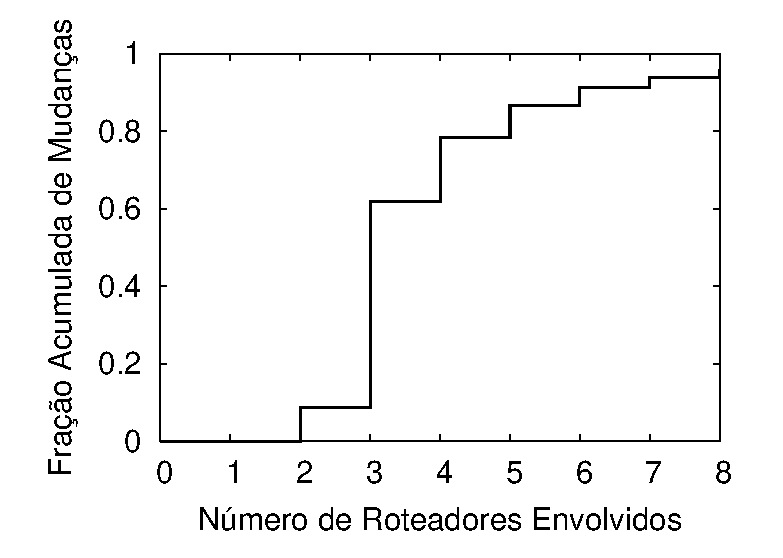
\includegraphics[width=0.47\textwidth]{figs/nrouters.eps}
\label{fig:char.nrouters}}
\hspace{2mm}
\subfigure[Distribuição da fração de roteadores de uma rota
envolvidos em mudanças de caminho]{
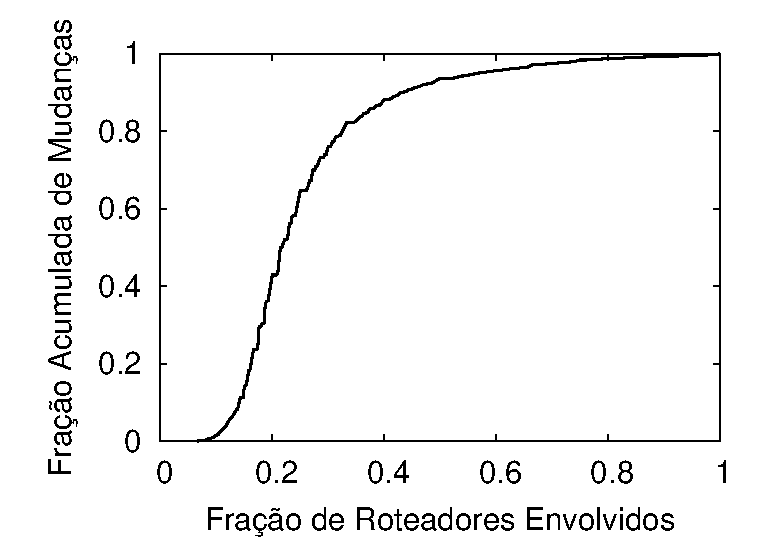
\includegraphics[width=0.47\textwidth]{figs/fracs.eps}
\label{fig:char.fracs}}
\vspace{-0.7em}
\caption{Caracterização de mudanças de caminho na Internet}
\label{fig:char}
\vspace{-0.4em}
\end{center}
\end{figure}

A \figstr~\ref{fig:char.fracs} mostra a distribuição da fração de saltos
de um caminho envolvidos numa mudança, i.e., o número de roteadores
envolvidos na mudança dividido pelo tamanho da nova rota, para todas as
mudanças nos nossos dados.  Vemos que 76\% das mudanças de caminho
envolvem menos de 30\% dos saltos no caminho.  Isso mostra o potencial
do remapeamento local para redução de sondas de medição, se comparado
com a abordagem atual de remapear o caminho por inteiro.  A curva começa
em $x = 0.066 = 2/30$ acontece porque uma mudança envolve pelo menos
dois saltos e porque o \dtrack{} só mede os 30 primeiros saltos num
caminho (o padrão do traceroute e do Paris
traceroute~\cite{jacobson1989traceroute, augustin07}).

A \figstr~\ref{fig:char.nasns} mostra a distribuição do número de
sistemas autônomos envolvidos em mudanças de caminho.  Convertemos
endereços IPs medidos pelo \dtrack{} em sistemas autônomos combinando as
tabelas de mapeamento do Team Cymru\footnotemark{} e
iPlane~\cite{madhyastha06iplane}.  Cada endereço IP que não aparece na
tabela de mapeamento combinada é associado a um sistema autônomo que
contém apenas um endereço IP.  Essa é uma medida conservadora que pode
sobrestimar o número de sistemas autônomos envolvidos em uma mudança.
A \figstr~\ref{fig:char.nasns} explica porque mudanças de roteamento
envolvem poucos saltos.  Mesmo fazendo a conversão de endereços IP para
sistemas autônomos de forma conservadora, vemos que 60\% das mudanças de
caminho é interna a um sistema autônomo e apenas 7\% envolve mais de
dois sistemas autônomos.

\footnotetext{Team Cymru, IP to ASN Mapping,
{http://www.team-cymru.org/Services/ip-to-asn.html}}

\begin{figure}[t]
\begin{center}
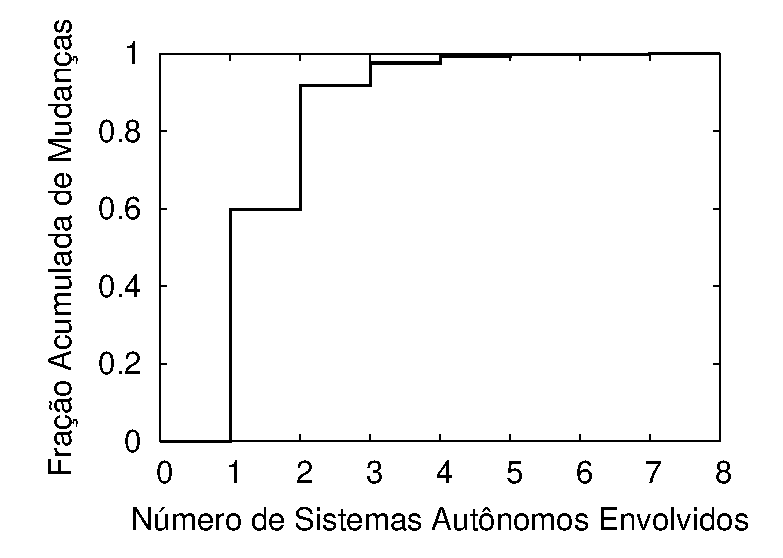
\includegraphics[width=0.47\textwidth]{figs/nasns.eps}
\caption{Distribuição do número de sistemas autônomos envolvidos em
mudanças de caminho}
\label{fig:char.nasns}
\end{center}
\end{figure}
